\section{Comportamiento}
A continuación se describe el comportamiento de los diferentes componentes del sistema. Estos diagramas son basados en el trabajo realizado por \cite{tesis-meneses-sebastian} y \cite{tesis-cerda-rodrigo}, dado que se busca replicar el comportamiento del sistema en dispositivos móviles.

\subsection{Obtener guantes}

\begin{figure}[H]
  \begin{center} 
   	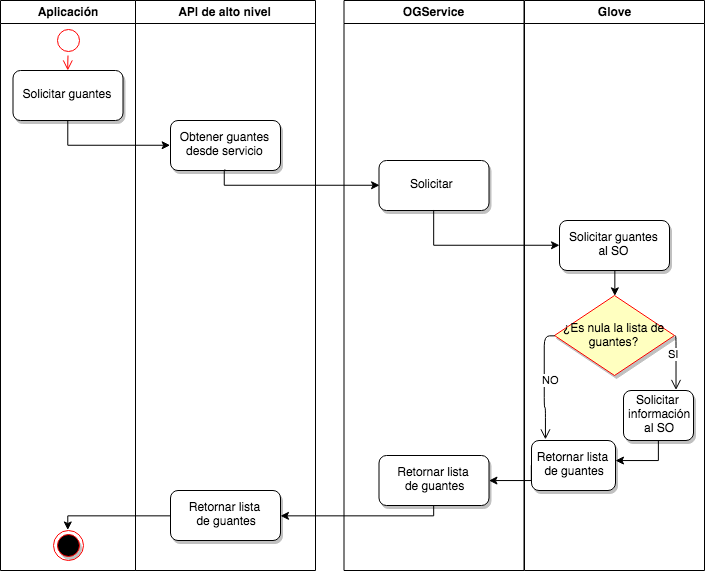
\includegraphics[width=1.0\textwidth]{images/chapter04/ActivityDiagrams-GetGloves.png} 
    \caption[Obtener guantes]{Obtener guantes \\Fuente: Elaboración propia (2018)}
    \label{fig:activity-diagrams01-GetGloves}
  \end{center}
\end{figure}

\subsection{Activación}

\begin{figure}[H]
  \begin{center} 
   	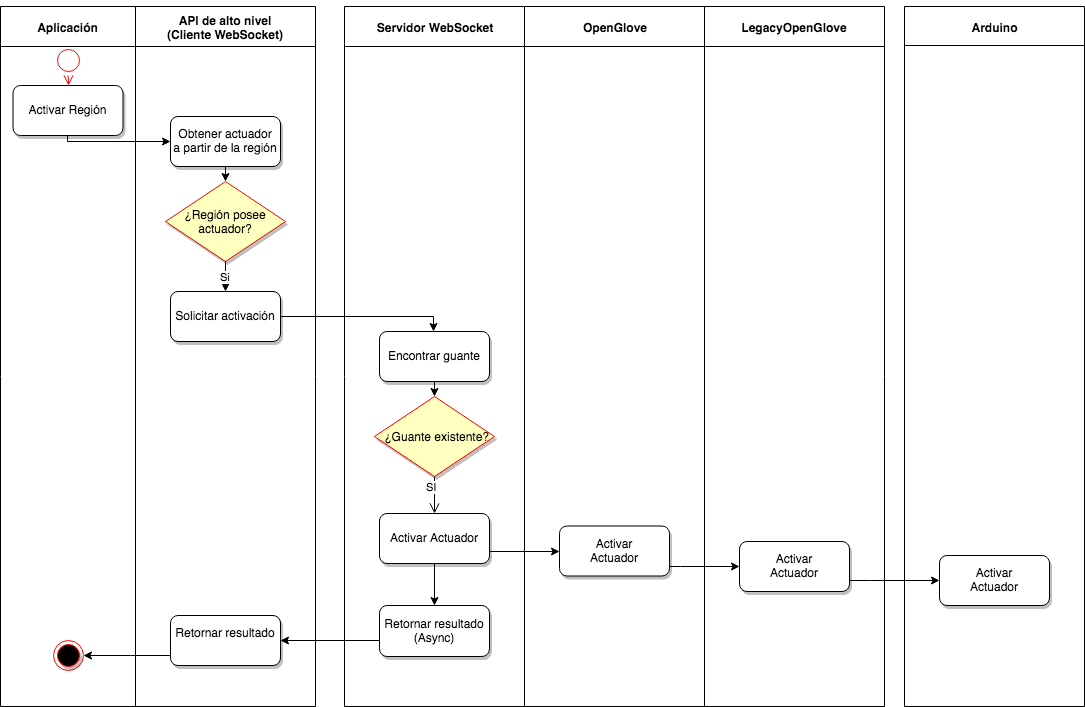
\includegraphics[width=1.0\textwidth]{images/chapter04/ActivityDiagrams-RegionActivation.png} 
    \caption[Activar región]{Activar región \\Fuente: Elaboración propia (2018)}
    \label{fig:activity-diagrams02-RegionActivation}
  \end{center}
\end{figure}

\subsection{Añadir flexor a una región}

\begin{figure}[H]
  \begin{center} 
   	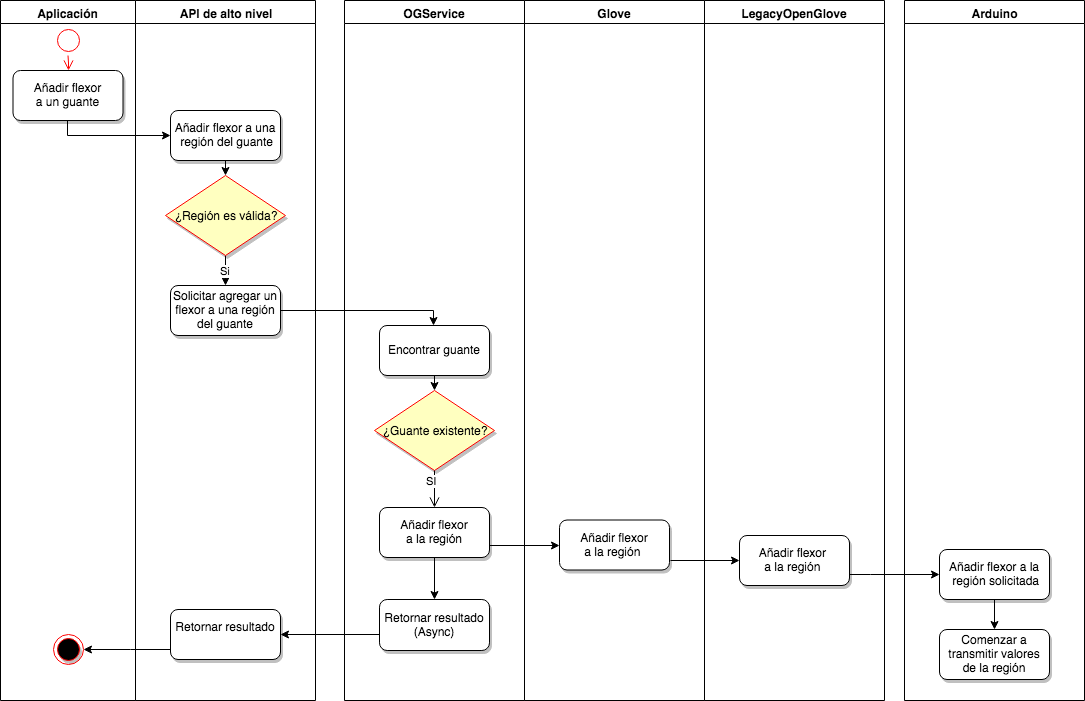
\includegraphics[width=1.0\textwidth]{images/chapter04/ActivityDiagrams-AddFlexorToRegion.png} 
    \caption[Agregar flexor a una región]{Agregar flexor a una región \\Fuente: Elaboración propia (2018)}
    \label{fig:activity-diagrams03-AddFlexorToRegion}
  \end{center}
\end{figure}

\subsection{Asignar Threshold}

\begin{figure}[H]
  \begin{center} 
   	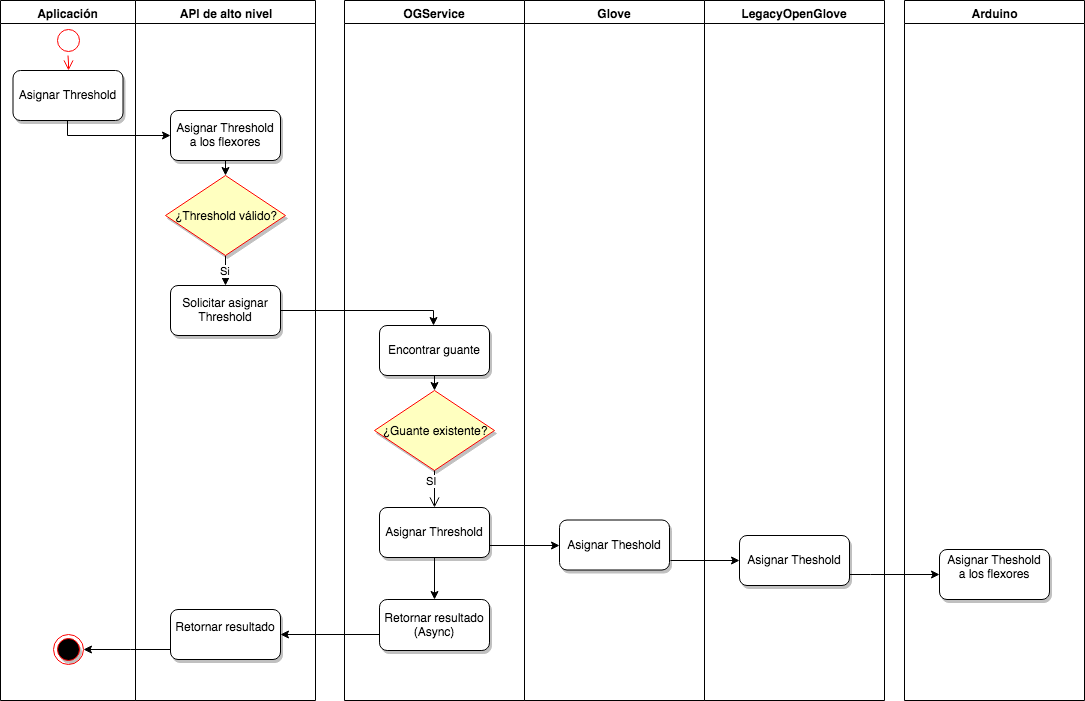
\includegraphics[width=1.0\textwidth]{images/chapter04/ActivityDiagrams-AssignThreshold.png} 
    \caption[Asignar Threshold]{Asignar Threshold \\Fuente: Elaboración propia (2018)}
    \label{fig:activity-diagrams04-AssignThreshold}
  \end{center}
\end{figure}

\subsection{Iniciar IMU}

\begin{figure}[H]
  \begin{center} 
   	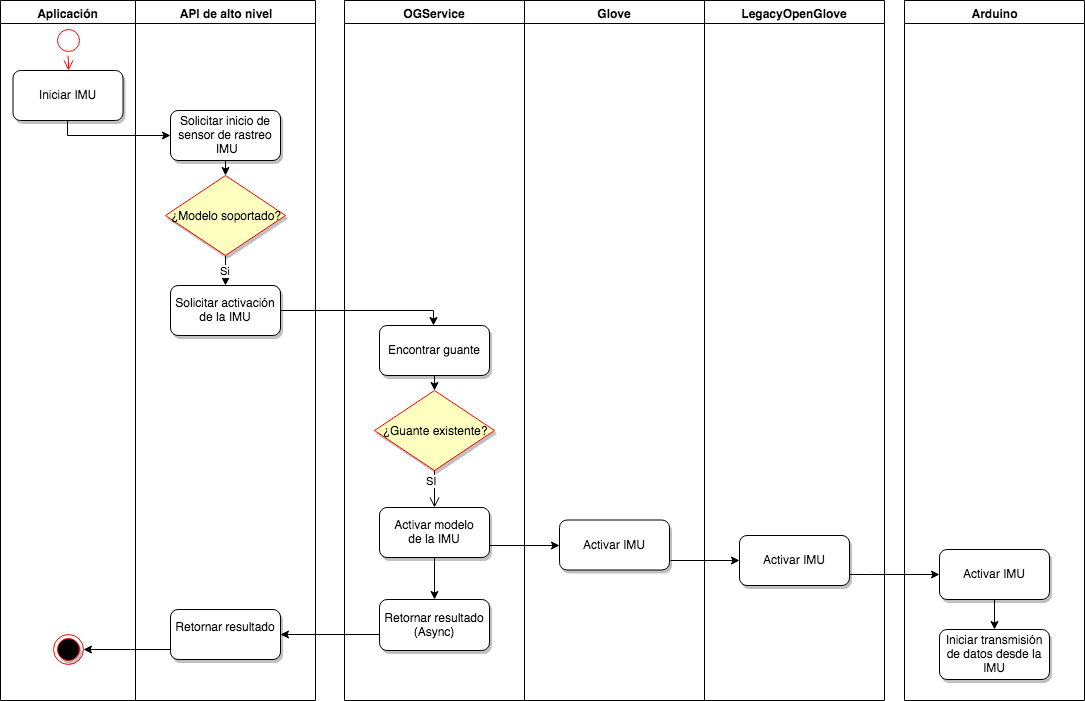
\includegraphics[width=1.0\textwidth]{images/chapter04/ActivityDiagrams-StartIMU.png} 
    \caption[Iniciar IMU]{Iniciar IMU \\Fuente: Elaboración propia (2018)}
    \label{fig:activity-diagrams05-StartIMU}
  \end{center}
\end{figure}

\subsection{Lectura de datos provenientes de Arduino}

\begin{figure}[H]
  \begin{center} 
   	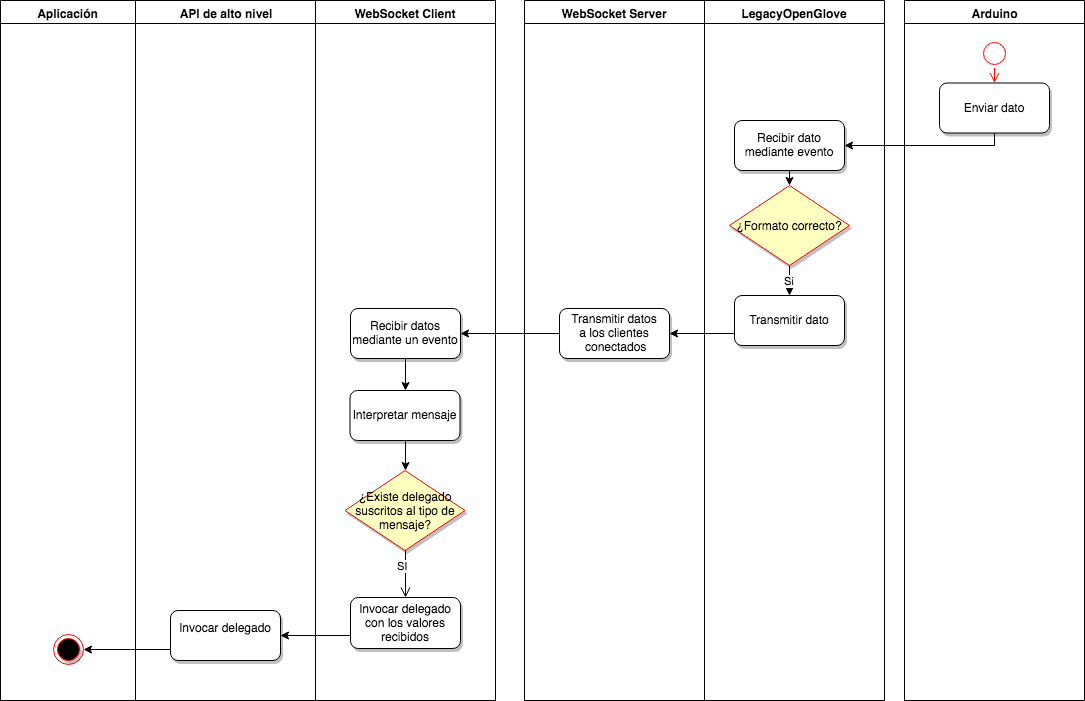
\includegraphics[width=1.0\textwidth]{images/chapter04/ActivityDiagrams-ReadDataFromArduino.png} 
    \caption[Lectura de datos provenientes de Arduino]{Lectura de datos provenientes de Arduino \\Fuente: Elaboración propia (2018)}
    \label{fig:activity-diagrams06-ReadDataFromArduino}
  \end{center}
\end{figure}